\documentclass[tikz, border=4pt]{standalone}
\usepackage{tikz}
\usepackage{pgfplots}
\pgfplotsset{compat=1.18}
\begin{document}
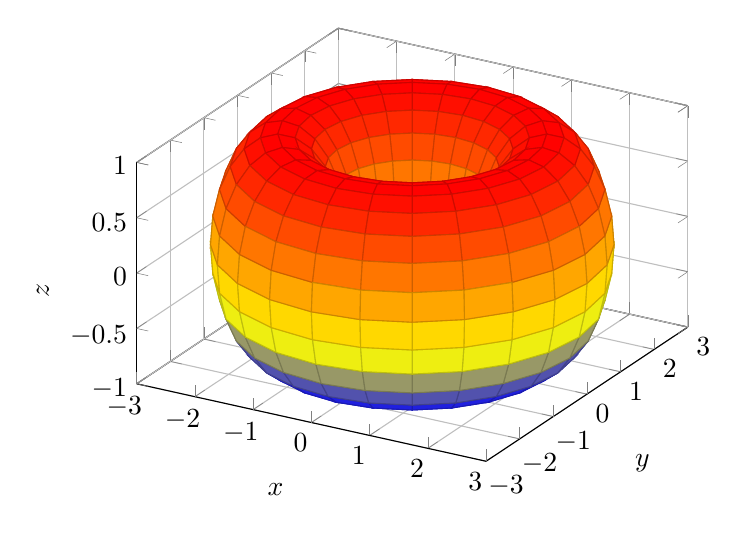
\begin{tikzpicture}[x=1cm, y=1cm]
  \definecolor{tdc1}{HTML}{1E5BD6}

  \begin{axis}[
    at={(0cm,-5.5cm)},
    anchor=south west,
    scale only axis,
    width=7cm,
    height=5.5cm,
    xmin=-3,
    xmax=3,
    ymin=-3,
    ymax=3,
    zmin=-1,
    zmax=1,
    view={30}{35},
    xtick={-3,-2,-1,0,1,2,3},
    ytick={-3,-2,-1,0,1,2,3},
    ztick={-1,-0.5,0,0.5,1},
    grid=major,
    xlabel={$x$},
    ylabel={$y$},
    zlabel={$z$}
  ]
    \addplot3[surf, shader=faceted, z buffer=sort, domain=0:6.2832, y domain=0:6.2832, samples=25, forget plot] ({((2+cos(deg(y)))*cos(deg(x)))}, {((2+cos(deg(y)))*sin(deg(x)))}, {sin(deg(y))});
  \end{axis}
\end{tikzpicture}
\end{document}
